\chapter{$tt\bar{H}$ 分析结果}\label{chap:ttH_results}

\section{\ltwotau 结果}
首先忽略归一化或者形状影响低于0.5\%的系统误差,最终考虑的系统误差如图~\ref{Fig:1l2tau.pruning}所列。图~\ref{Fig:1l2tau.nuispar}展示冗余参数拟合前和拟合后对信号强度的影响($\theta_{fit}-\theta_{0}/\Delta\theta$);图~\ref{Fig:1l2tau.asimov}给出拟合前和拟合后BDT的分布。最终给出的期望信号强度为:$$\mu_{ttH}=1.00^{+0.88}_{-0.75}(Stat)^{+0.85}_{-0.69}(syst)=1.00^{+1.22}_{-1.02}(total)$$,对应0.98个标准偏差。系统误差间的相关性和系统误差影响排序如图~\ref{Fig:1l2tau.impacts}所示,最大的误差是假$\tau_{had}$的统计误差。

\begin{figure}[htbp]
\centering
\begin{center}
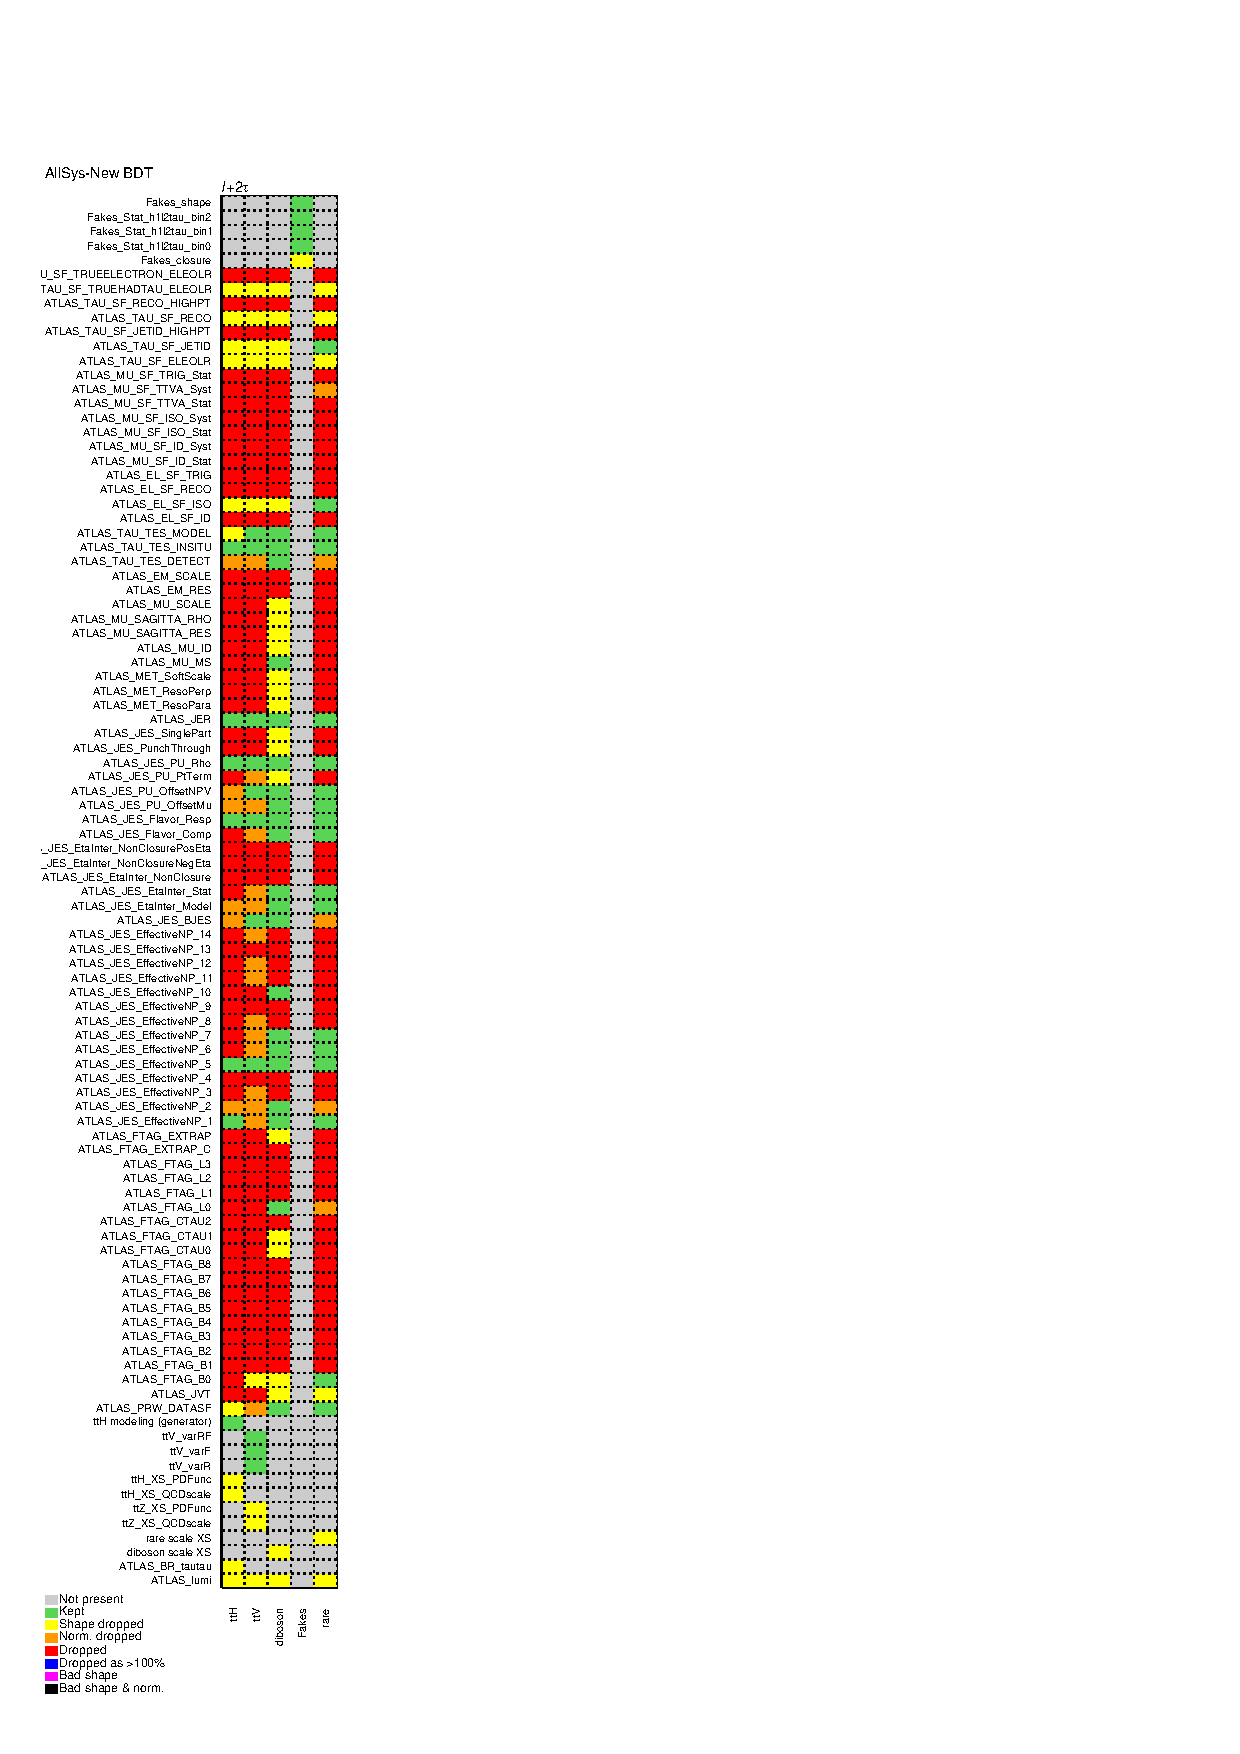
\includegraphics[width=0.35\textwidth, height=0.8\textheight]{fig/OneLepTwoTaus/Pruning.pdf}
\end{center}
\caption{The systematics used in the \texttt{fitter}.}
\label{Fig:1l2tau.pruning}
\end{figure}

\begin{figure}[htbp]
\centering
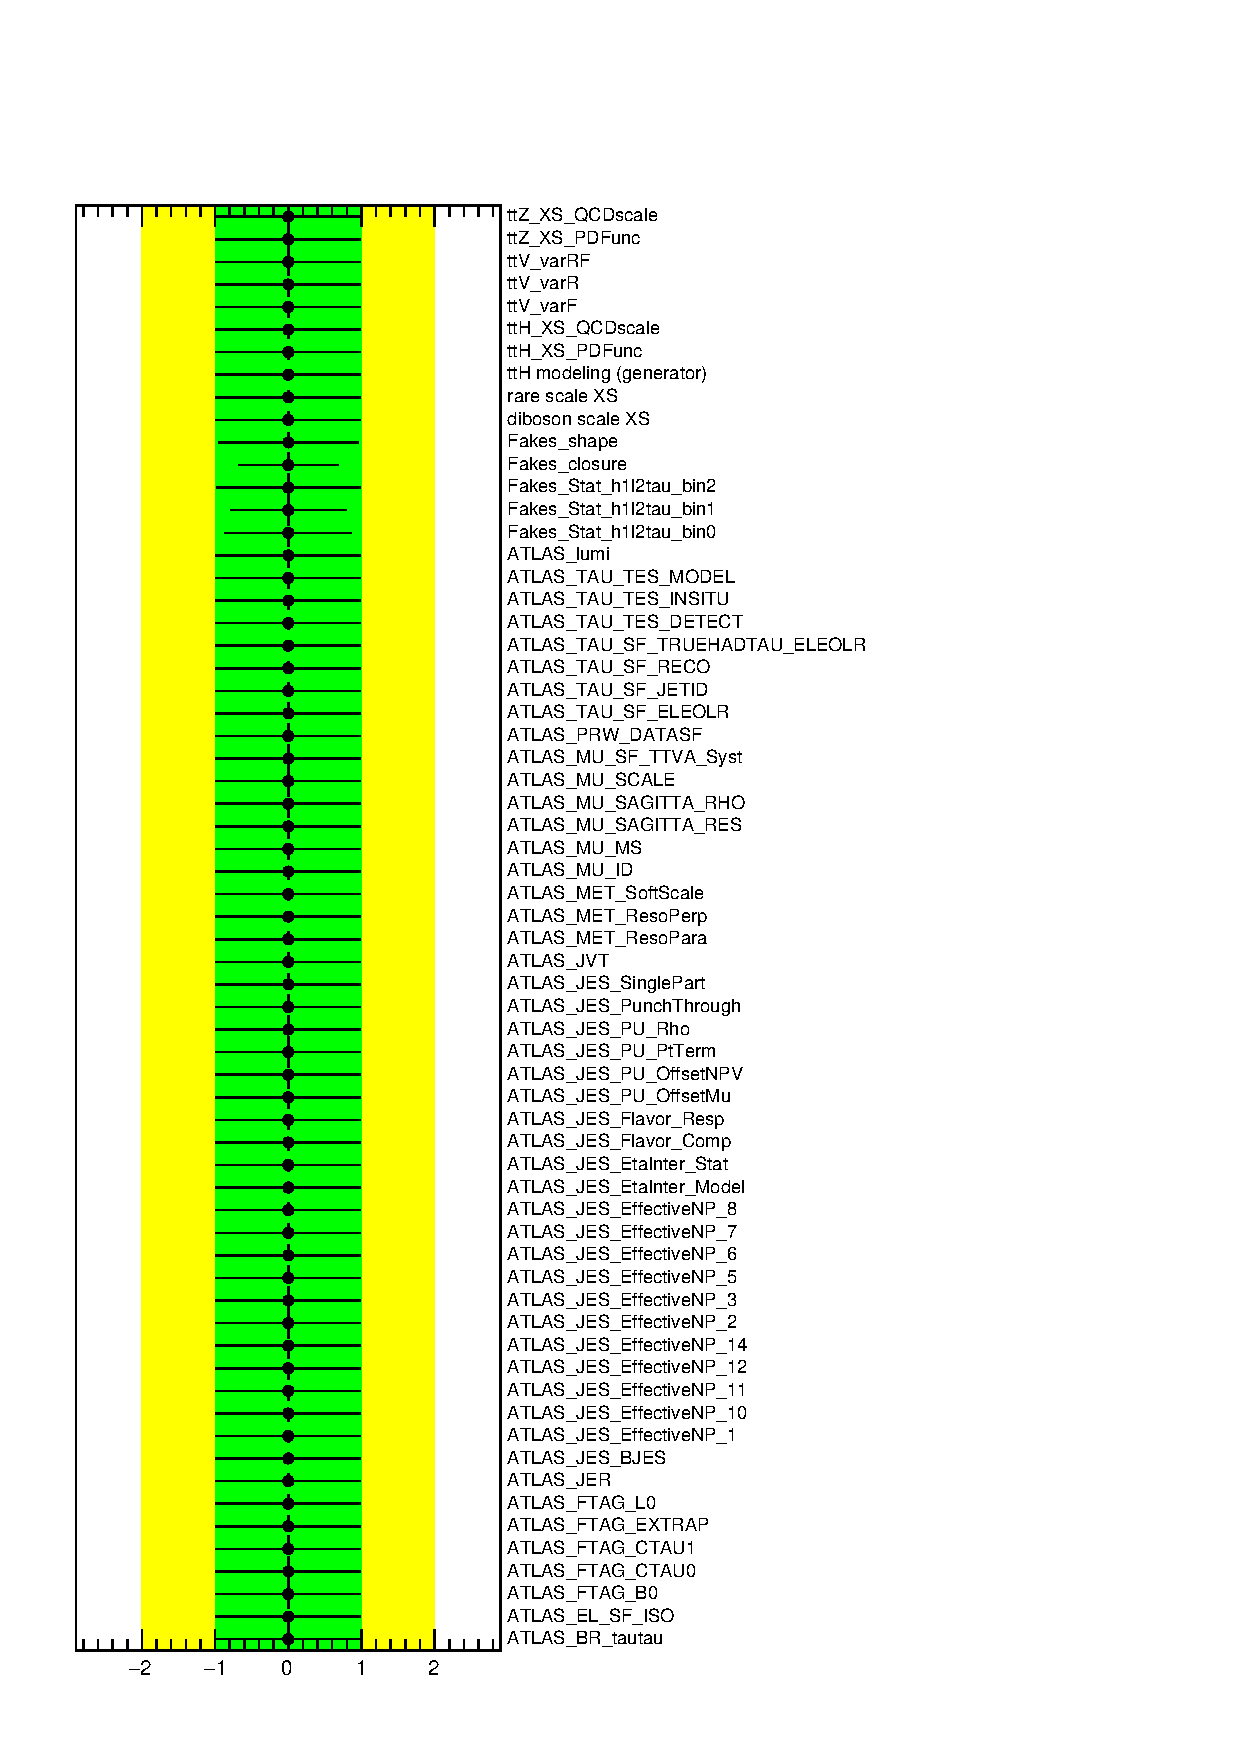
\includegraphics[width=0.7\textwidth, keepaspectratio]{fig/OneLepTwoTaus/NuisPar.pdf}
\caption{The pull plot for systematics.}
\label{Fig:1l2tau.nuispar}
\end{figure}

\begin{figure}[htbp]
\centering
\begin{center}
  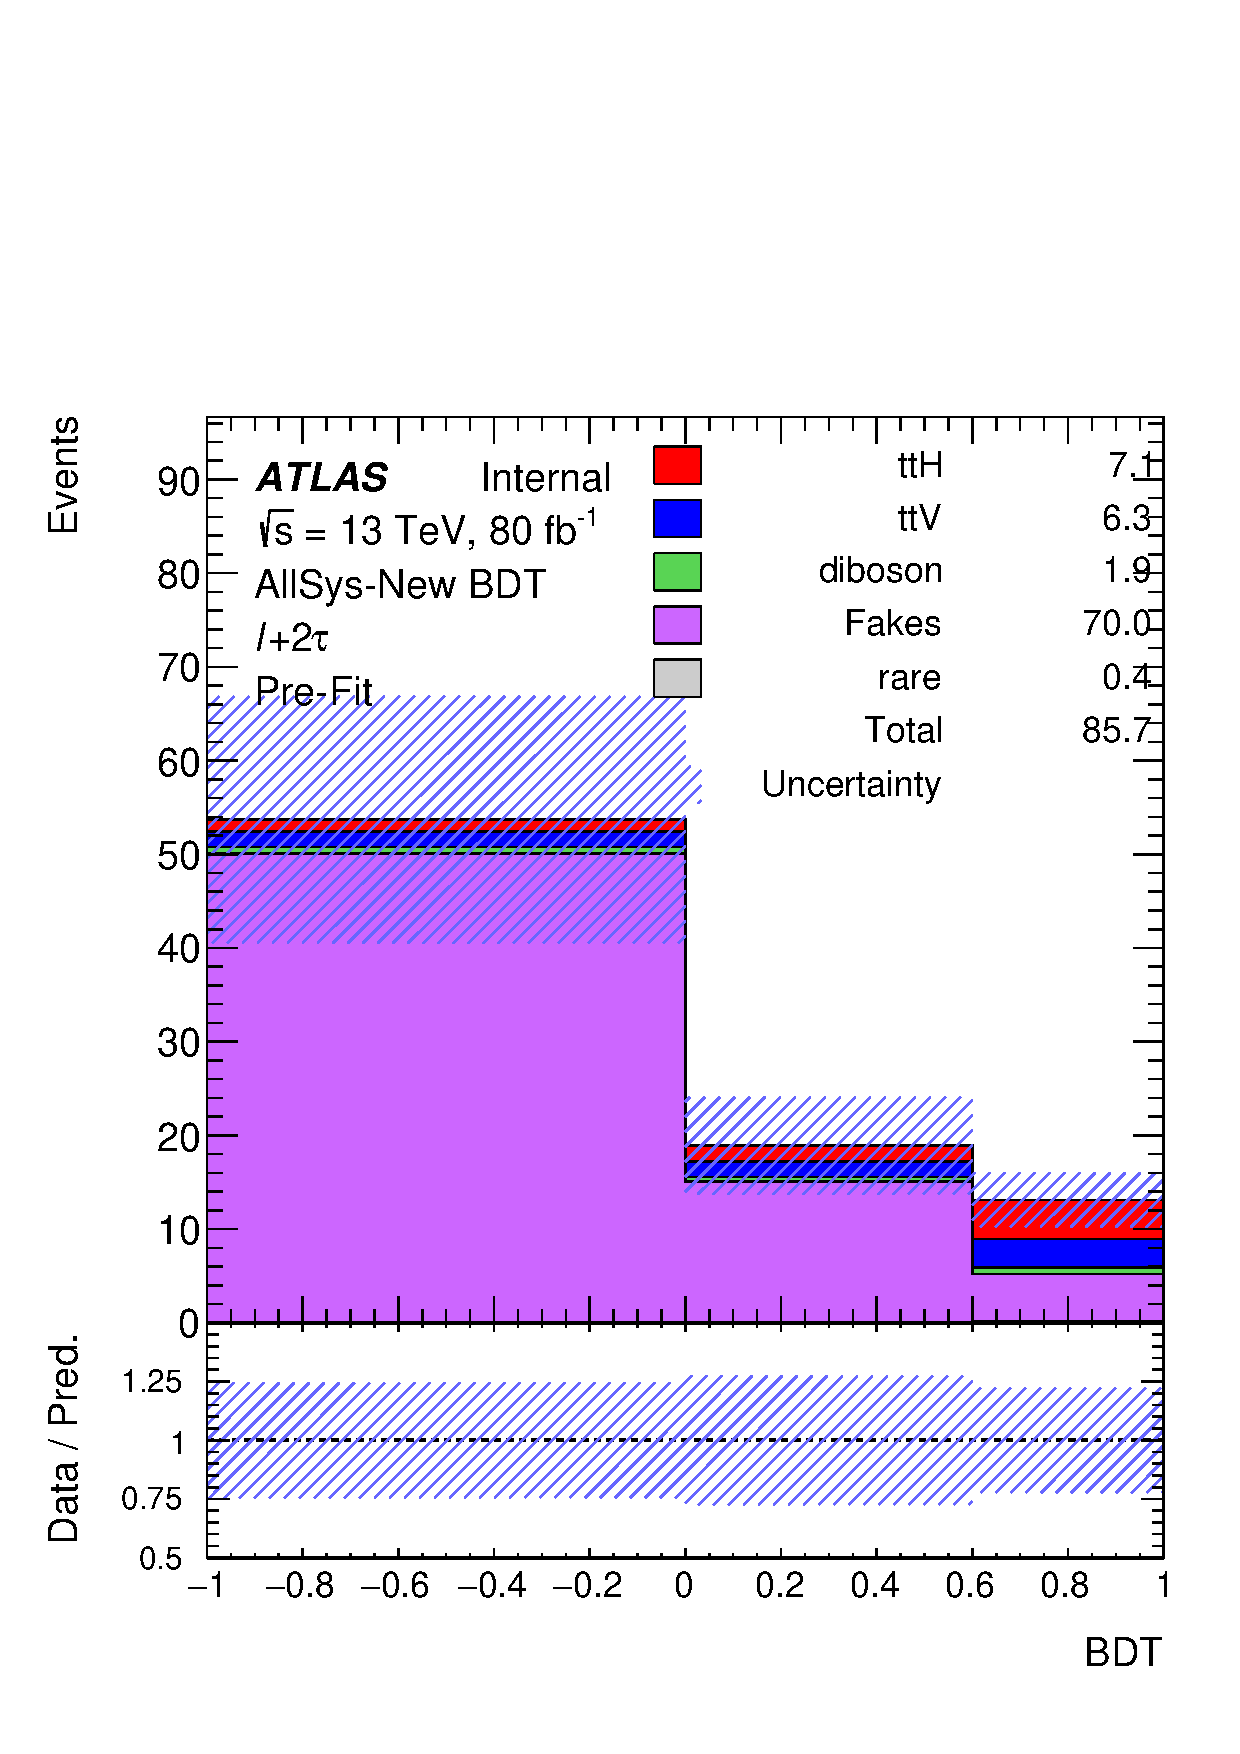
\includegraphics[width=0.45\textwidth, keepaspectratio]{fig/OneLepTwoTaus/h1l2tau.pdf}
  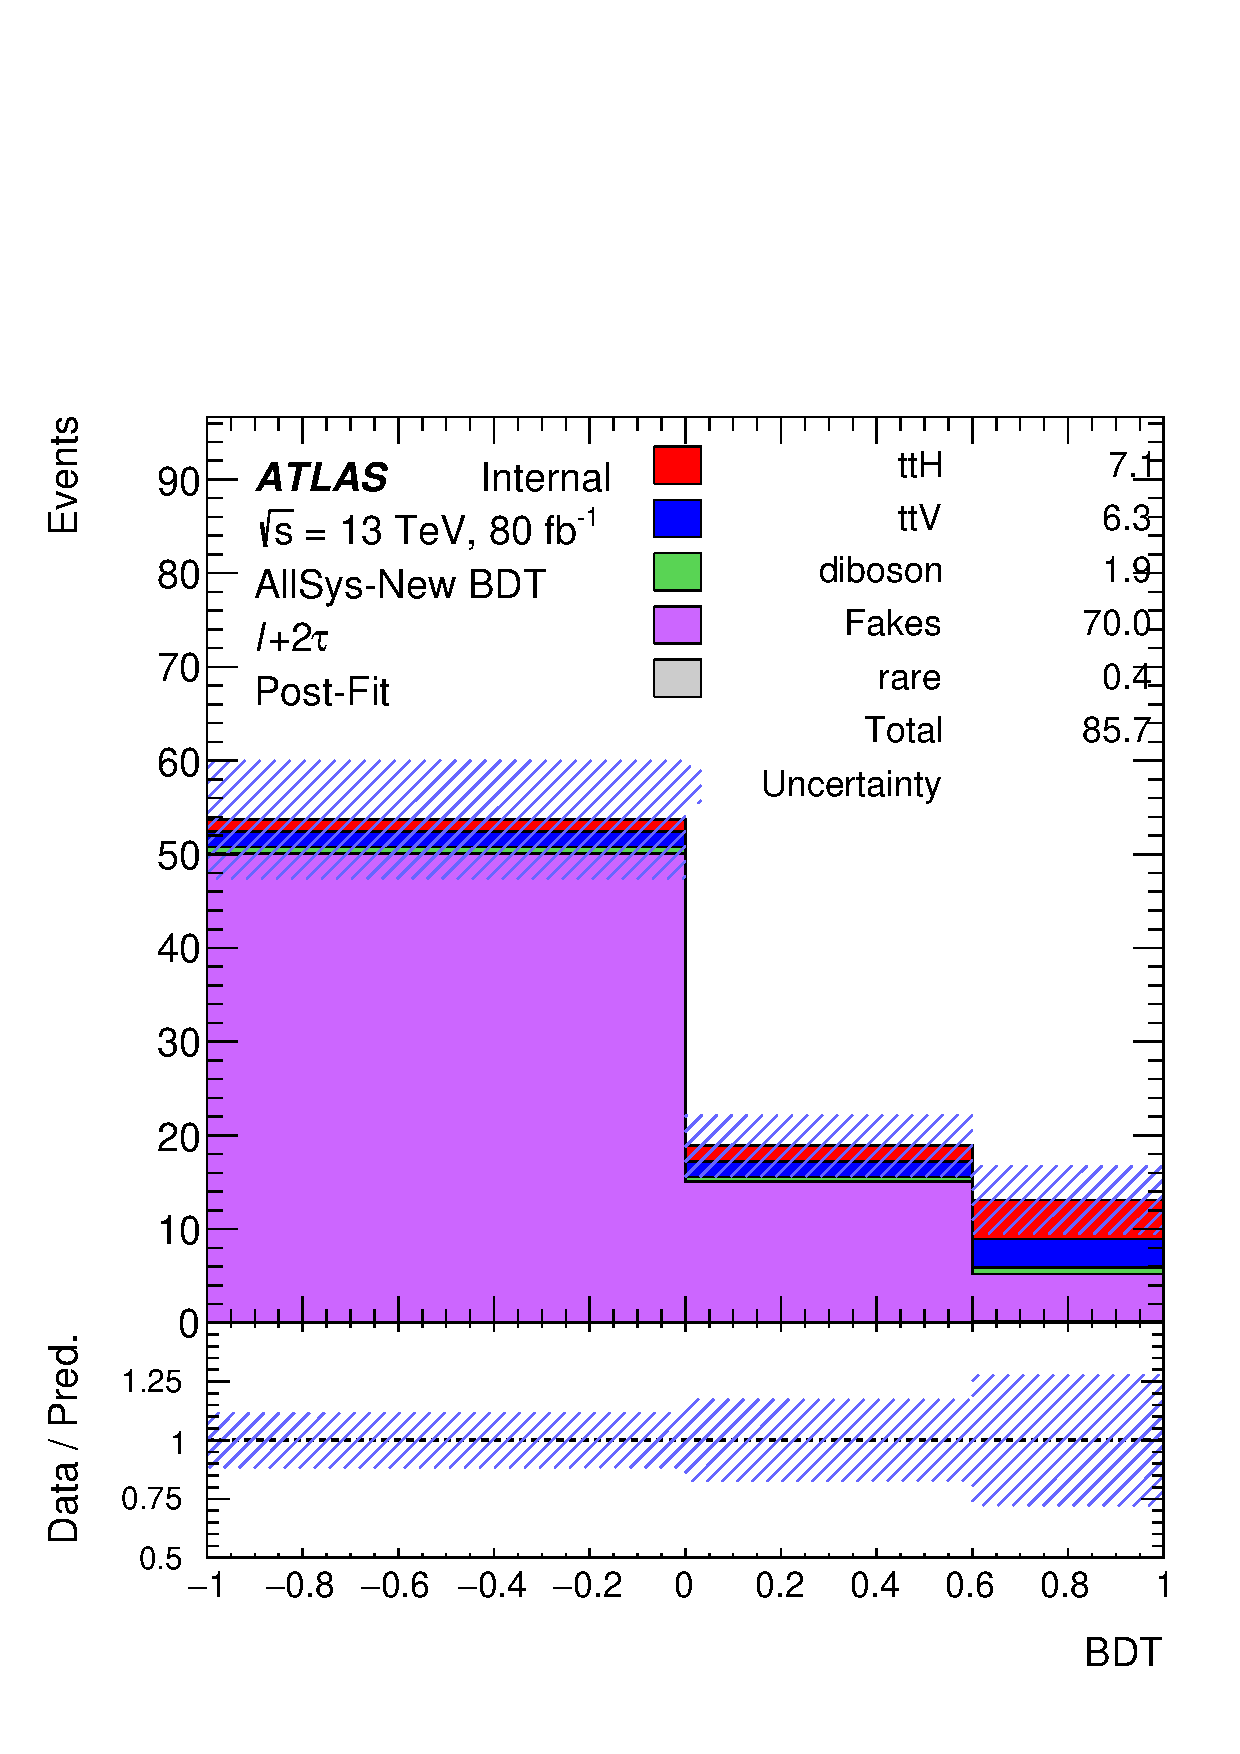
\includegraphics[width=0.45\textwidth, keepaspectratio]{fig/OneLepTwoTaus/h1l2tau_postFit.pdf}
\end{center}
\caption{The BDT Asimov data are shown in pre-fit (left) and post-fit (right). 
%({\bf update})
}
\label{Fig:1l2tau.asimov}
\end{figure}

\begin{figure}[htbp]
\centering
\begin{center}
  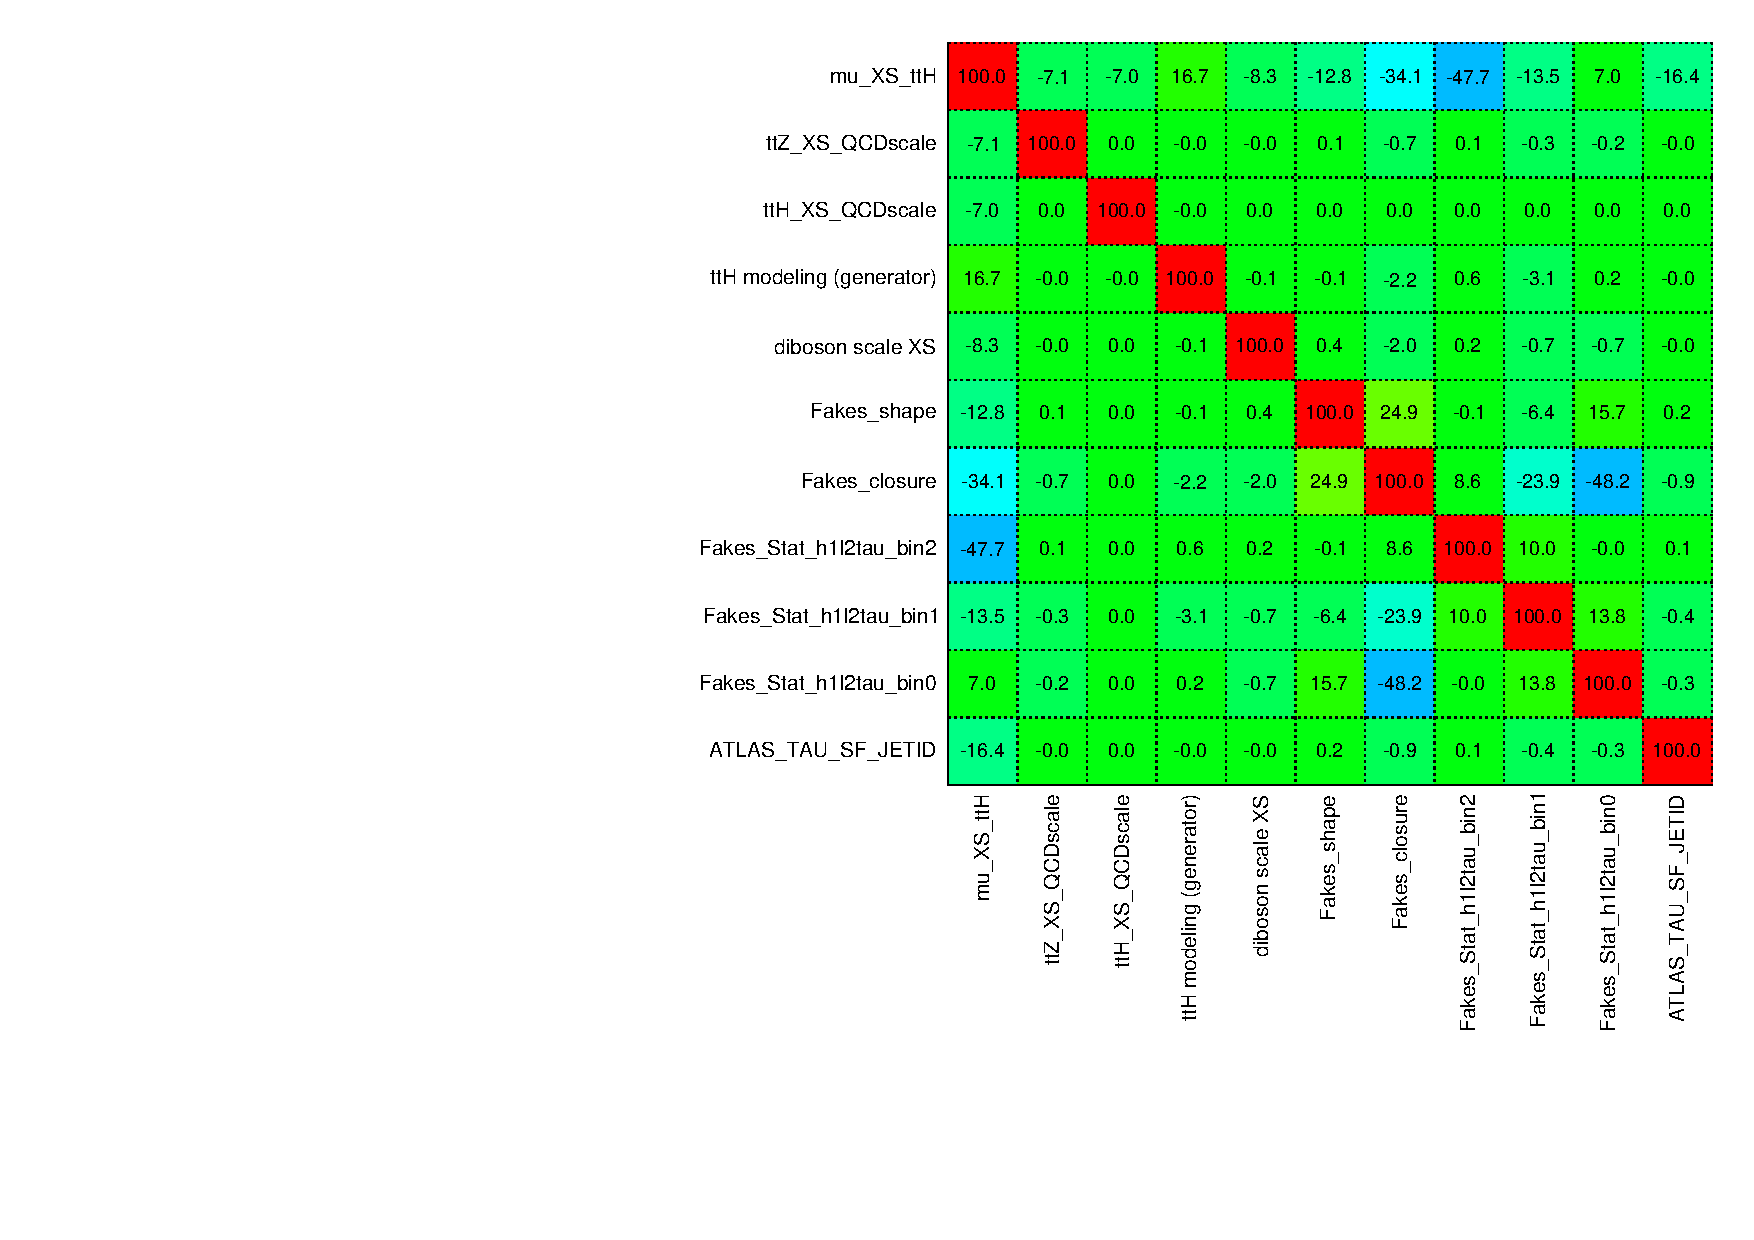
\includegraphics[width=0.45\textwidth, keepaspectratio]{fig/OneLepTwoTaus/CorrMatrix.pdf}
  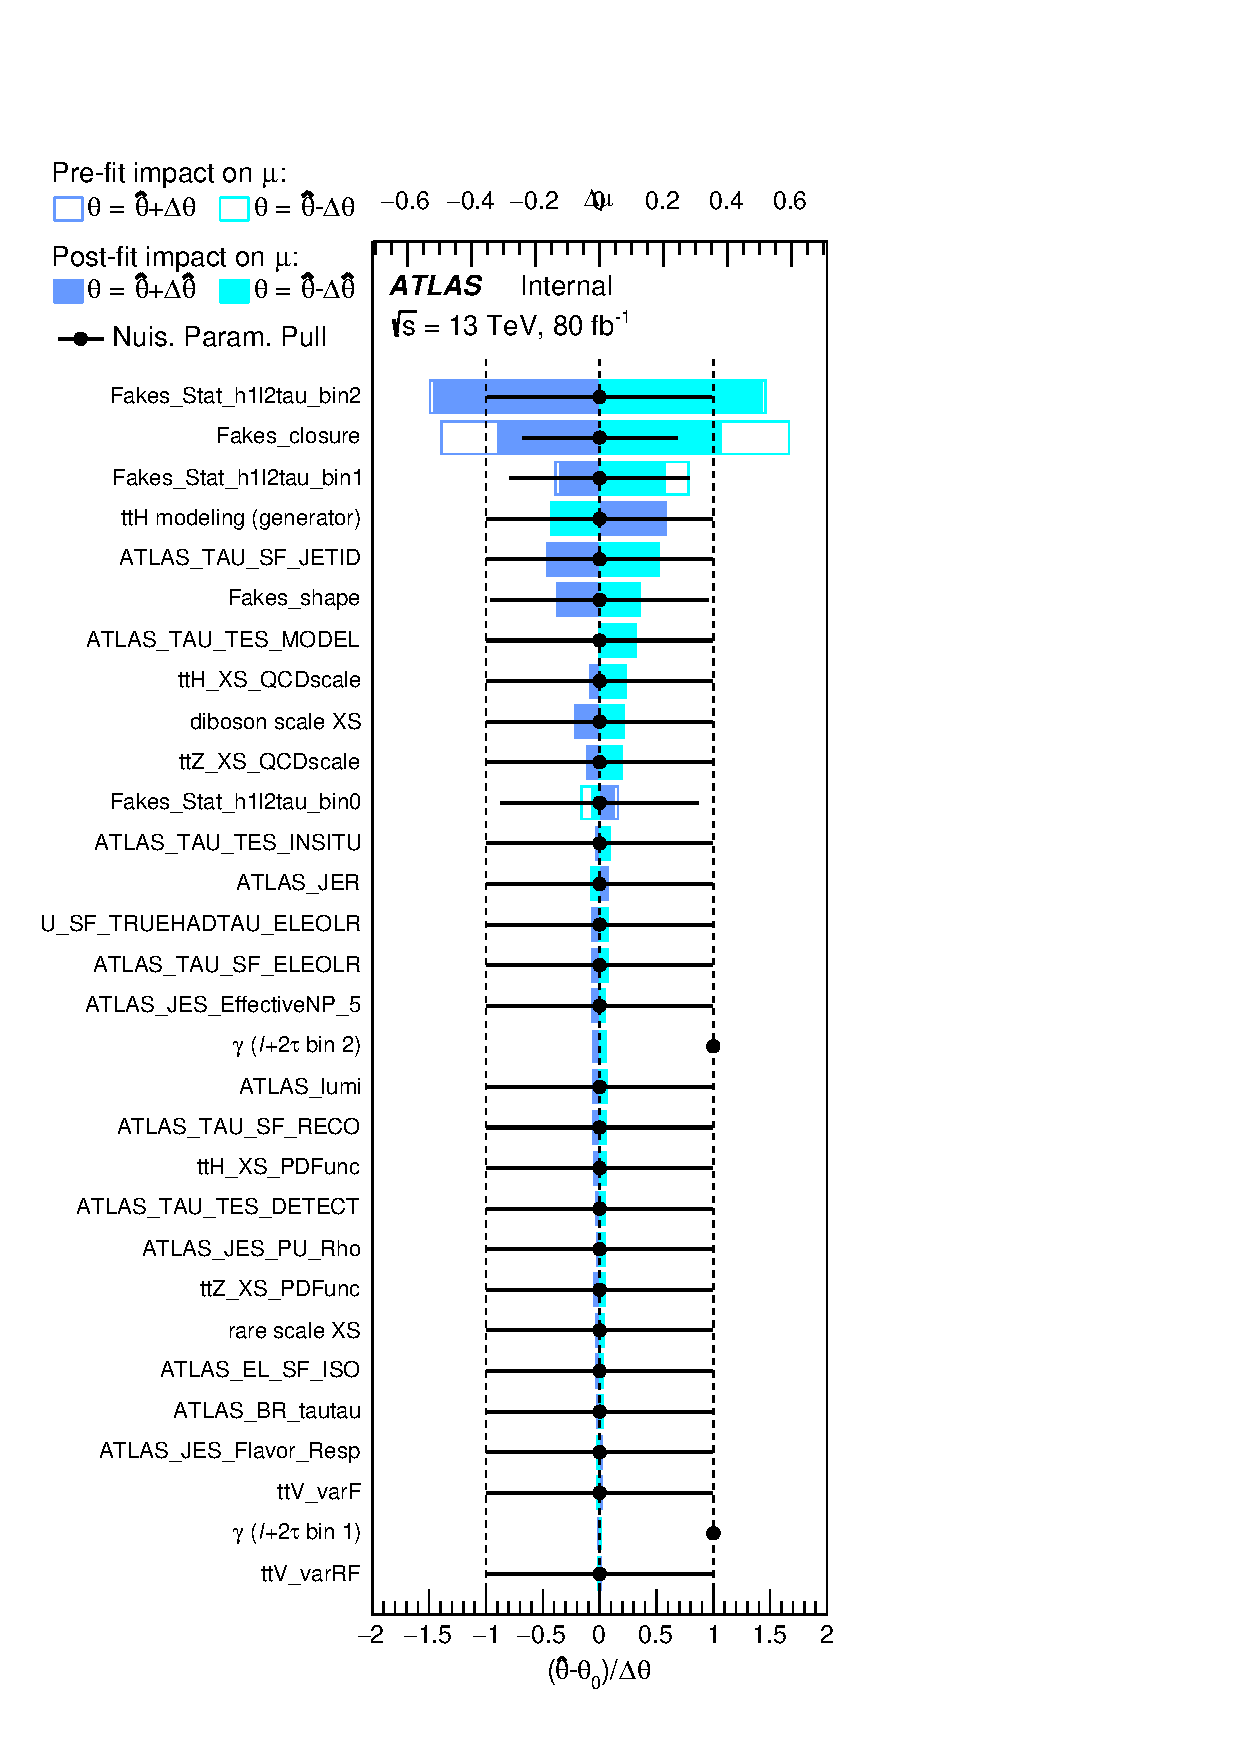
\includegraphics[width=0.5\textwidth, keepaspectratio]{fig/OneLepTwoTaus/Ranking.pdf}
\end{center}
\caption{Left: the fitted correlation; Right: ranking of systematic based on their impacts on the signal strength measurements. 
%({\bf update})
}
\label{Fig:1l2tau.impacts}
\end{figure}